\documentclass[11]{article}
\usepackage[tmargin=1 in,bmargin=1 in,lmargin=0.5 in,rmargin=0.5 in]{geometry}
\usepackage{graphicx}
\usepackage{amssymb}
\usepackage{url}

\begin{document}

\title{Physics Behind the Simulation:A CS296 Group 15 Report}
\author{Abhishek Gupta\\
110040067\\
\texttt{abhishek.10004@gmail.com}\\
\and Praneeth Naidu\\
110050046\\
\texttt{svpraneethnaidu@gmail.com}\\
\and Mayank Dehgal\\
110050024\\
\texttt{mayankdehgal94@gmail.com}}
\date{January 25, 2013}
\maketitle

\section{Introduction}
This report is done as a part of Software Systems Lab assignment which focuses on learning\cite{webTut} LaTeX.This report contains the explanation of three top level elements in the design of \emph{Rube Goldberg Machine} in \emph{cs296\_basecode}. The following section deals with the \textbf{physics} involved in those three top level elements in the design

\section{Physics Behind the Simulation}
\subsection{Pendulum Bob and the Dominos}
The very first action in the design is, a pendulum bob hits a domino which eventually collapses the series of dominos placed one by one. When the bob hits the first domino, an impulsive force causes the first domino to rotate about the point that is touching the ground.
\begin{center}
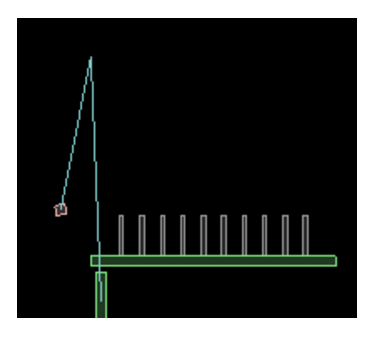
\includegraphics[scale=0.6]{1}
\end{center}
\begin{equation}
\int F.dt=mv
\end{equation} 
where $\int F.dt$($Newton.second$) is the \textit{Impulse}, $m$($Kg$) is the \textit{Moment of Inertia} and $v$($rad/sec$) is the \textit{Velocity at point of contact}

\subsection{Collision of Balls}
The collision of balls is related to the concept of \emph{Conservation of Momentum}
\begin{center}
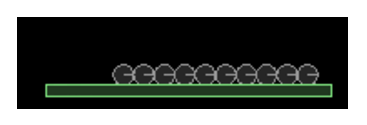
\includegraphics[scale=0.6]{2}
\end{center}
When two bodies of masses $m_{1}(Kg)$ and $m_{2}(Kg)$, moving with velocities $u_{1}(m/s)$ and $u_{2}(m/s)$ respectively collide with each other,
\begin{equation}
m_{1}u_{1}+m_{2}u_{2}=m_{1}v_{1}+m_{2}v_{2}
\end{equation}
where $v_{1}(m/s)$ and $v_{2}(m/s)$ are their \textit{final velocities} respectively.
\newline

In this design, \textit{coefficient of restitution = 0} which \textit{implies} final velocities of both the bodies are same\cite{collision} and the second body is at rest and let the mass of each ball be $m$.
\begin{equation}
\therefore mu_{1}=2mv
\Rightarrow v=\frac{u_{1}}{2} m/s
\end{equation} 
where $v$ is the final velocity of the combined mass $2m$.In this way, the velocity keeps reducing by a factor of 2 with each collision which eventually leads to a very very slow velocity.


\subsection{Pulley Arrangement}
The arrangement shown  in the figure involves very basic \emph{Newton's laws of motion}. When sufficient weight is loaded on to the left basket, the right basket rises up and then the expected further actions will take place.
\begin{center}
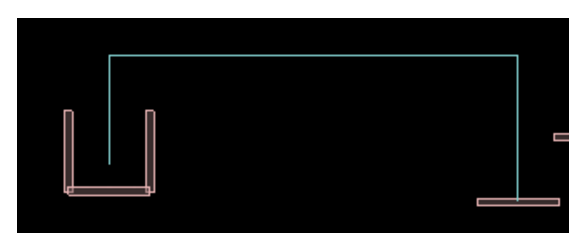
\includegraphics[scale=0.6]{3}
\end{center}
\begin{equation}
F-T = m_{1}a
\end{equation}
\begin{equation}
T-m_{2}g = m_{2}a
\end{equation}
where $F$($N$) is the \textit{pulling force on left basket}, $m_{1}$($Kg$) and $m_{2}$($Kg$) are \textit{masses of the bodies in left and right baskets} respectively , $T$($N$) is the \textit{tension in the thread} and $a$($m/s^2$) is the \textit{acceleration with which the bodies move} in the system.

If $F$ is considered to be $m_{1}g$, from above equations, we get
\begin{equation}
\therefore a=\frac{(m_{1}-m_{2})g}{m_{1}+m_{2}} m/s^2
\end{equation}
In this way, the plank on right attains some velocity because of this acceleration and can hit/push objects as per the design.
\section{Conclusions}
As we have seen above, \textbf{Physics} is involved in almost every aspect of the machine. In Section 2.1 we have seen the \textbf{Impulse-Momentum} concept. In Section 2.2 we have seen the \textbf{Conservation of Momentum} concept. In Section 2.3 we have seen the \textbf{Laws of Motion} concept. In this way, each segment of the machine is using a specific part of physics which emphasizes the importance of physics in designing machines\cite{dummy}.

\bibliographystyle{unsrt}
\bibliography{report_cs296_15_bib}

\end{document}
